\FloatBarrier
\section{Baseline Model Capacity (Simultaneous, Heterogeneous Dimensions)}
Before beginning to evaluate this model on the sequential benchmark described above, we wanted to verify it has the capacity to learn our intended task in a non-meta-learning context. We trained different variants of the model described above on the entire training set, evaluating the model on all single-item queries on every image on the test set after each epoch. We reasoned that in order to merit investigating meta-learning using this model, we should first prove it has the capacity to solve these tasks in an easier setting. We term this condition as simultaneous (rather than sequential), heterogeneous dimensions (using queries from all three dimensions, rather than homogeneous conditions, which use queries from a single dimension).

The initial dataset we generated included 4096 stimuli (split 7/8'ths training and 1/8'th test), using eleven shapes and ten colors, and without querying on materials, since at the time we only had two of them (the two we inherited from CLEVR). The model as described above failed to learn the task well and overfit the training set. Figure \ref{fig:results-baseline-initial-dataset} demonstrates such overfitting, evidenced by a plateau in the test set loss (left) and accuracy (right), while the performance on the training set continues to improve.

\begin{figure}[!htb]
% \vspace{-0.225in}
\centering
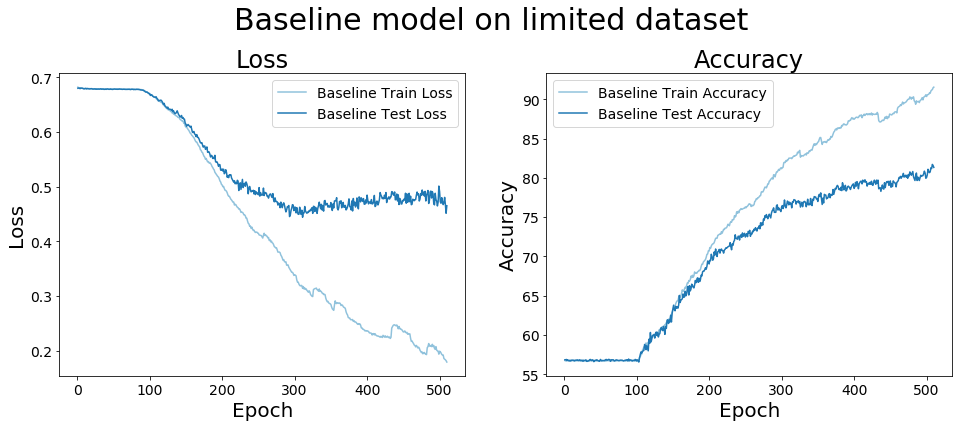
\includegraphics[width=\linewidth]{ch-results/figures/baseline/initial_dataset.png}
\caption{{\bf Baseline model on initial dataset.} This model shows substantial overfitting, evidenced by the stagnation in test set metrics while the training set metrics continue improving.}
\label{fig:results-baseline-initial-dataset}
% \vspace{-0.2in}
\end{figure}

These concerns were alleviated when we successfully generated the final, full dataset, which includes an order of magnitude more images (45,000 training, 5000 test), as well as the final collection of shapes, colors, and materials we intended to use. In an attempt to quantify performance better, we switched from accuracy to another measure, the AUC ROC (area under the receiver operating characteristic curve), which considered the performance of the model across different decision thresholds. Whereas the accuracy is computed with a fixed decision threshold between classifying as positive and negative, usually 0.5, the ROC score is computed by comparing the false-positive and true-positive range across all possible threshold values, from zero to one, providing a more holistic measure of the model’s success. Figure \ref{fig:results-baseline-full-dataset} plots the performance of the baseline model described above, without any measures to aid generalization and prevent overfitting, on the full dataset. It proved far more successful in learning the task when trained on the full dataset, even if it did show some overfitting. 

\begin{figure}[!htb]
% \vspace{-0.225in}
\centering
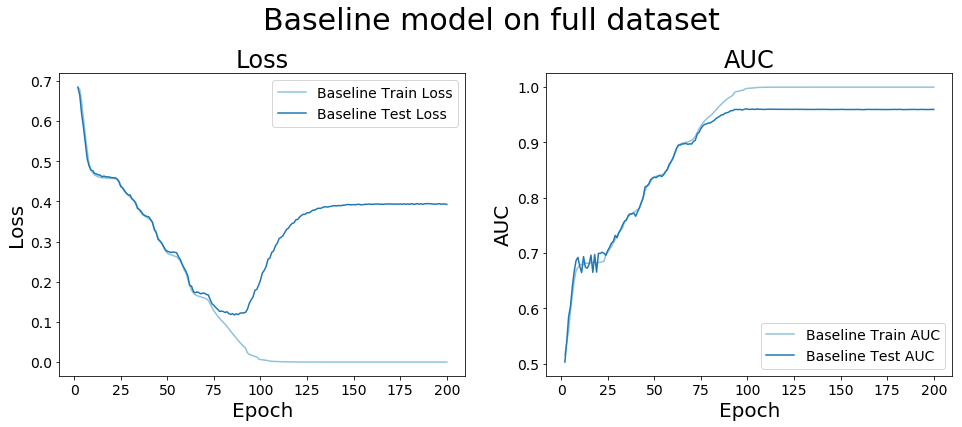
\includegraphics[width=\linewidth]{ch-results/figures/baseline/full_dataset.png}
\caption{{\bf Baseline model on full dataset.} This model still shows some evidence of overfitting, but with a much better overall performance on both the training and test sets.}
\label{fig:results-baseline-full-dataset}
% \vspace{-0.2in}
\end{figure}

In an attempt to alleviate the overfitting, we experimented with two fairly standard modifications, as outlined in the Section \ref{ch:models-compared}. Figure \ref{fig:results-baseline-anti-overfitting} provides the results from adding dropout to the fully connected layers, and adding weight decay to the entire model. Both were added in tandem with allowing the learning rate to drop if the loss fails to improve for ten consecutive epochs. We were surprised to discover that despite the prevalence of dropout in the literature, it failed to learn well in this task; we might have investigated why, but having discovered that weight decay works spectacularly well, we opted to use it instead. Training with dropout, the loss peaks higher, the AUC does not reach 0.70, whereas training with weight decay goes about as ideally as one could imagine:

\begin{figure}[!htb]
% \vspace{-0.225in}
\centering
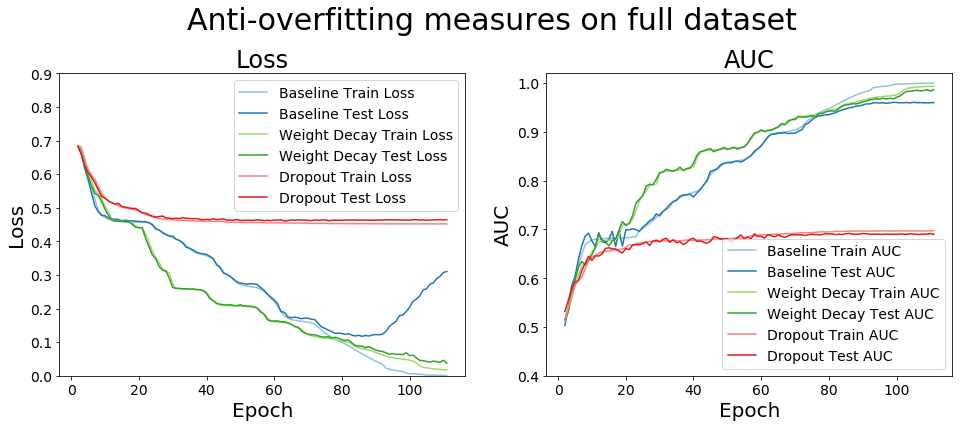
\includegraphics[width=\linewidth]{ch-results/figures/baseline/full_dataset_anti_overfitting.png}
\caption{{\bf Anti-overfitting measures on full dataset.} Adding weight decay drastically improves performance, while adding dropout causes the model to stagnate much earlier.}
\label{fig:results-baseline-anti-overfitting}
% \vspace{-0.2in}
\end{figure}

While there is still a minor discrepancy between the test and train losses, it is minuscule compared to previous results, and the test accuracy and AUC peak higher with weight decay than without (without: accuracy 95.63\%, AUC 0.9607; with: accuracy 98.69\%, AUC 0.9905). We therefore employ this model with weight decay in all experiments reported below.
